\documentclass[12pt]{article}

\input{physicsPream}

%\setcounter{tocdepth}{1}

\begin{document}

%----------BEGIN TITLE----------

\begin{titlepage}

  \title{Experiment 1: Ray Optics}
  \author{Ryan Wojtyla \\
          Partner: Akshath Wikramanayake \\}
  \date{October 9, 2018}

\maketitle

\begin{center}
  Abstract
\end{center}

\qq During these experiments, we primarily investigated the reflection and
refraction of light, how lenses bend light, and the diffraction of
light. Several laws and principles, including Snell's Law and the Fundamental
Lens Equation, were validated through the collection and processing of data.

\thispagestyle{empty}

\end{titlepage}

%-----------END TITLE-----------

%\tableofcontents

\section{Experiments}

%----------BEGIN EXPERIMENT 1----------

\subsection{Experiment 1: Introduction to Ray Optics}

\subsubsection{Sketch}

\begin{figure}[H]
  \label{pic:exp1}
  \begin{center}
    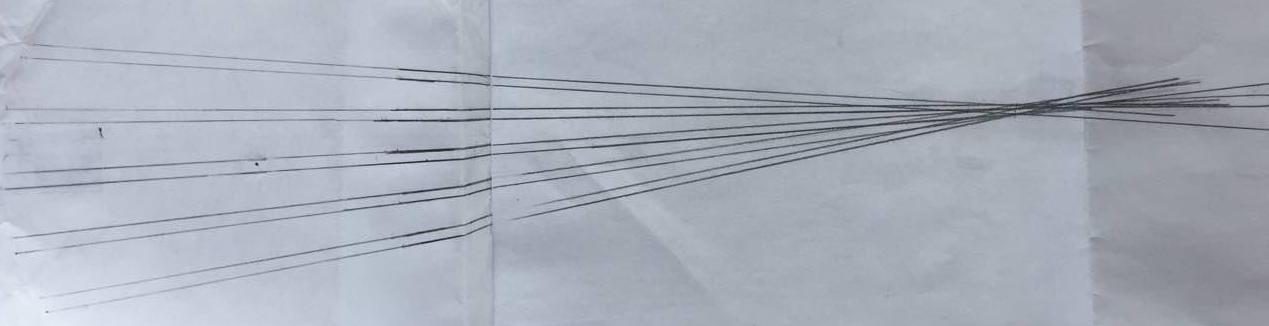
\includegraphics[scale=0.3]{exp1.jpg}
  \end{center}
  \caption{Tracing the divergent rays back to the light source.}
\end{figure}

\subsubsection{Straight Line Propagation of Light}

\subsubsubsection{}

While the rays are straight, they are not parallel with each other.

\subsubsubsection{}

As the rays' distance from the Slit Plate increases, their width increases while
their distinctness decreases.

\subsubsubsection{}

All of the rays appeared to originate from the Light Source, even when viewed
from a slight angle.

\subsubsubsection{}

As the angle of the Slit Plate increases, becomes more horizontal, the width of
the rays increases while their distinctness decreases.

\subsubsubsection{}

The images are most distinct when the Slit Plate is entirely vertical, and
they are least distinct when it is horizontal.

\subsubsection{Ray Tracing: Locating the Filament}

\subsubsubsection{}

The distance between the reference mark in the center of the Ray Table and the
point of intersection of the rays at the filament
is \(d_e = 24.1 \pm 0.05 \si{\centi\meter}\).

\subsubsubsection{}

The distance between the filament and the center of the Ray Table was measured
to be \(d_t = 25.6 \pm 0.05 \si{\centi\meter}\).

\subsubsubsection{}

The two measurements have a percent error, where
\(\%_{err} = \frac{|d_t - d_e|}{d_t} \cdot 100\%\), of \(\%_{err} = 5.86\%\), and a percent
uncertainty, where \(\delta \%_{err} = \frac{\%_{err}}{d_e}\), of \(\delta
\%_{err} = 0.249 \%\). Although the percent error, \(5.86\% \pm 0.249\%\), is low,
it is, nonetheless, present.

%-----------END EXPERIMENT 1-----------

%----------BEGIN EXPERIMENT 2----------

\subsection{Experiment 2: The Law of Reflection}

\subsubsection{Data}

\begin{figure}[H]
  \label{tab:2.1}
  \caption{\textbf{Table 2.1:} The two angles of reflection compared to their
    corresponding angle of incidence in degrees.}
  \begin{center}
    \begin{tabular}{|c|c|c|}
      \hline
      Incidence & Reflection\(_1\) & Reflection\(_2\) \\
      \hline
      0 & 0 & 0 \\   
      10 & 10 & 10 \\
      20 & 20 & 20 \\
      30 & 30 & 30 \\
      40 & 40 & 40 \\
      50 & 50 & 50 \\
      60 & 60 & 60 \\
      70 & 70 & 70 \\
      80 & 80 & 80 \\
      90 & 90 & 90 \\
      \hline
    \end{tabular}
  \end{center}
\end{figure}

\subsubsection{Questions}

\subsubsubsection{}

The results of the two trials are the same.

\subsubsubsection{}

The incident ray, reflected ray, and normal all lie on the same plane because
the reflected and incident rays are visible on the 2D surface of the Ray
Table. Because they are both visible on the 2D surface, they must both reside in
the same 2D plane.

\subsubsubsection{}

The angle of incidence and the angle of reflection are both the same value. 
 
%-----------END EXPERIMENT 2-----------

%----------BEGIN EXPERIMENT 3----------

\subsection{Experiment 3: Image Formation in a Plane Mirror}

\subsubsection{Sketch}

\begin{figure}[H]
  \label{pic:exp3}
  \begin{center}
    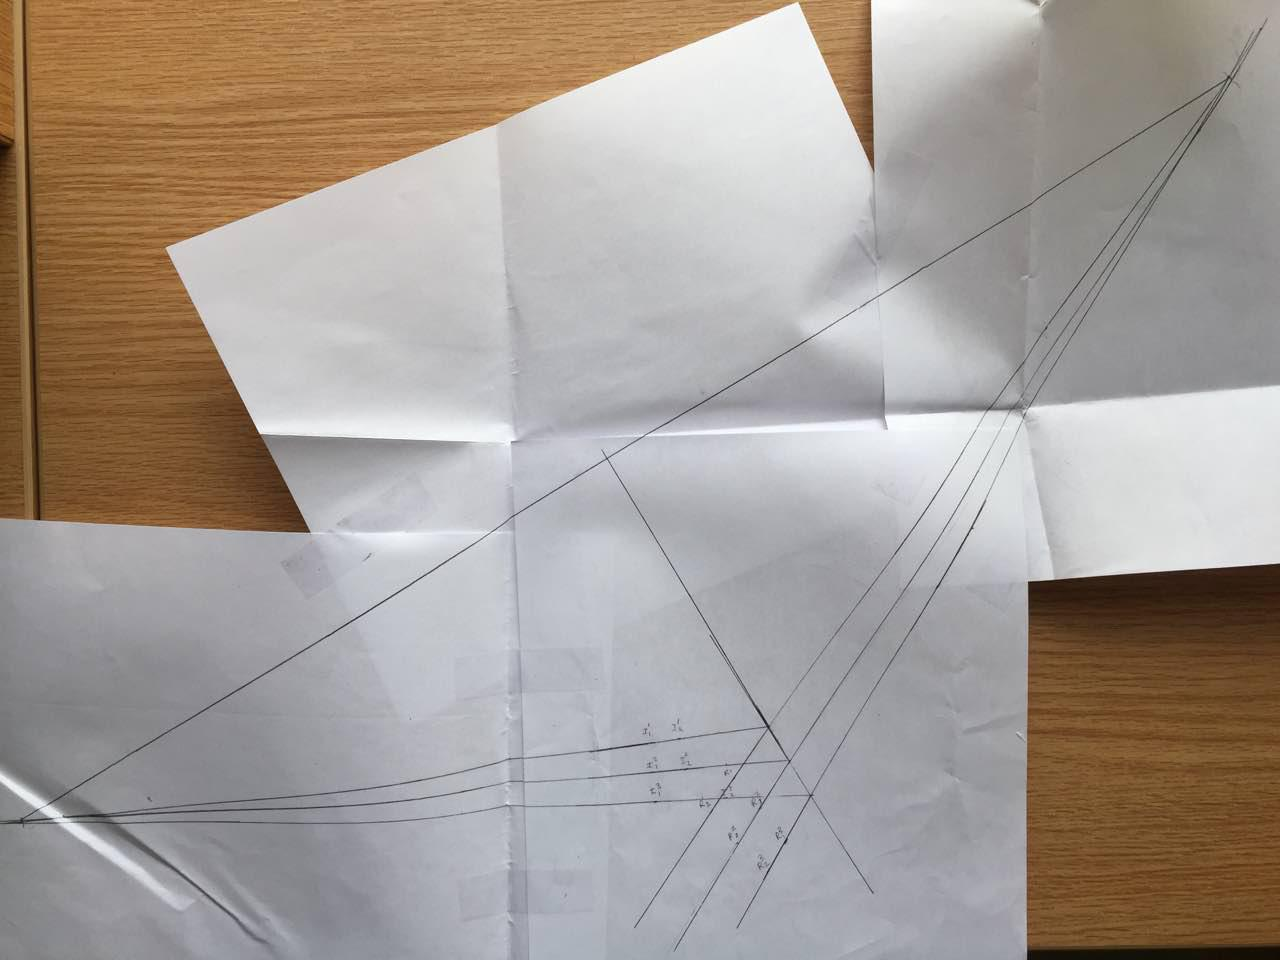
\includegraphics[scale=0.3]{exp3.jpg}
  \end{center}
  \caption{The tracing of the rays incident on the plane mirror.}
\end{figure}

\subsubsection{Questions}

\subsubsubsection{}

The rays do seem to follow a straight line into the mirror.

\subsubsubsection{}

The distance from the filament to the plane of the mirror (\(d_1\)) was measured
to be \(30.1 \pm 0.05 \si{\centi\meter}\).

\subsubsubsection{}

The perpendicular distance from the image of the filament to the plane mirror
(\(d_2\)) was measured to be \(30.0 \pm 0.05 \si{\centi\meter}\).

\subsubsubsection{}

The image will always appear to be the same distance away as if it were being
viewed straight on without a mirror.

%-----------END EXPERIMENT 3-----------

%----------BEGIN EXPERIMENT 4----------

\subsection{Experiment 4: The Law of Refraction}

\subsubsection{Data}

\begin{figure}[H]
  \label{tab:4.1}
  \caption{\textbf{Table 4.1:} The two symmetric angles of refraction from each
  angle of incidence. For angles of incidence \(\SI{80}{\degree}\) and
  \(\SI{90}{\degree}\), the ray internally reflected, so there were no
  refraction rays.}
  \begin{center}
    \begin{tabular}{|c|c|c|}
      \hline
      Incidence (\si{degree}) & Refraction\(_1\) (\si{degree}) &
                                                                 Refraction\(_2\)
                                                                 (\si{degree})
      \\
      \hline
      0  & 0    & 0 \\
      10 & 7    & 6 \\
      20 & 13   & 13 \\
      30 & 20   & 20 \\
      40 & 25   & 26 \\
      50 & 31.5 & 31.5 \\
      60 & 36   & 36 \\
      70 & 41.5 & 42 \\
      80 & n/a  & n/a \\
      90 & n/a  & n/a \\
      \hline
      \end{tabular}
      \end{center}
\end{figure}

\begin{figure}[H]
  \label{gph:exp4ref1}
  \begin{center}
    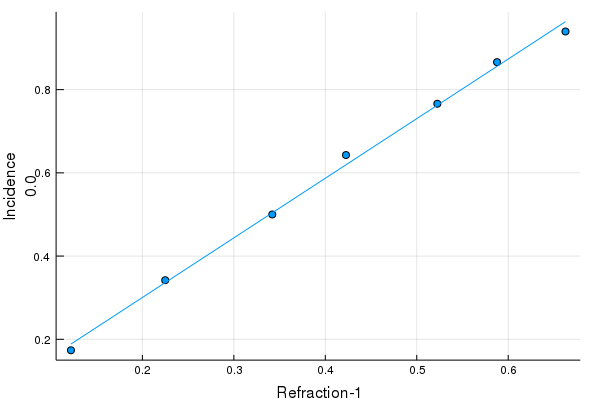
\includegraphics[scale=0.6]{exp4-ref1.png}
  \end{center}
  \caption{A graph where the x-axis is the sine of the first angle of refraction
    and the y-axis is the sine of the incidence angle. There is also a straight
    line of best fit.}
\end{figure}

\begin{figure}[H]
  \label{gph:exp4ref2}
  \begin{center}
    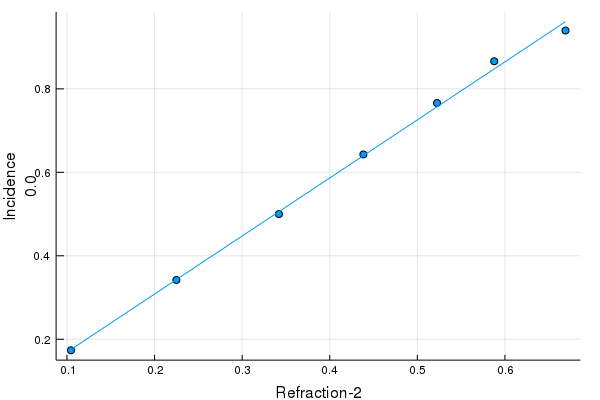
\includegraphics[scale=0.6]{exp4-ref2.png}
  \end{center}
  \caption{A graph where the x-axis is the sine of the second angle of refraction
    and the y-axis is the sine of the incidence angle. There is also a straight
    line of best fit.}
\end{figure}

\subsubsection{Questions}

\subsubsubsection{}

The ray is not bent when it passes into the lens perpendicular to the lens' flat
surface.

\subsubsubsection{}

The ray is slightly bent when it passes out of the lens perpendicular to the
lens' curved surface.

\subsubsubsection{}

While the two sets of measurements are very nearly identical, there are minor
differences between the two. These differences may be attributed to our
inability to perfectly align the ray with the Ray Table.

\subsubsubsection{}

The graphs are consistent with the Law of Refraction. The slopes are less than
one, which indicates that the medium, the lens, has a greater index of
refraction than the air from which the light originates. 

%-----------END EXPERIMENT 4-----------

%----------BEGIN EXPERIMENT 5----------

\subsection{Experiment 5: Reversibility}

\subsubsection{Data}

\begin{figure}[H]
  \label{tab:5.1}
  \caption{\textbf{Table 5.1:} The different angles, in degrees, of the light
    through two sides of the same medium.}
  \begin{center}
    \begin{tabular}{|c|c|c|c|}
      \hline
      Incidence\(_1\) & Refraction\(_1\) & Incidence\(_1\) & Refraction\(_2\) \\
      \hline
      0  & 0    & 0    & 0 \\
      10 & 6.5  & 6.5  & 11 \\
      20 & 12.5 & 12.5 & 20 \\
      30 & 20   & 20   & 30 \\
      40 & 25   & 25   & 40 \\
      50 & 31   & 31   & 47 \\
      60 & 37.5 & 37.5 & 58 \\
      70 & 43   & 43   & 74 \\
      80 & 45   & 45   & n/a \\
      \hline
    \end{tabular}
  \end{center}
\end{figure}

\subsubsection{Questions}

\subsubsubsection{}

The index of refraction for the acrylic, \(n_1\), can be found by using Snell's
Law, \(n_0 \sin{(\theta_i)} = n_1 \sin{(\theta_r)}\), rearranged as,
\(n_1 = \frac{n_0 \sin{(\theta_i)}}{\sin{(\theta_r)}}\). The value of \(n_1\)
was determined by calculating \(n_1\) for each of the
Incidence\(_1 = \theta_i\), Refraction\(_1 = \theta_r\) pairs, where
\(n_0 = 1\). The average of these values was then found to be \(n_1 =
1.48\). The first and last rows of data were removed from these calculations
because the first row is only zeros, and the last row contains a null value.

\subsubsubsection{}

Since now it is the destination index of refraction that is known, the formula
above must be rewritten as \(n_2 = \frac{n_0
  \sin{(\theta_r)}}{\sin{(\theta_i)}}\). The acrylic's index of
refraction was calculated using the same method as above, and the value was
found to be \(n_2 = 1.50\).

\subsubsubsection{}

The Law of Refraction is the same for rays entering and exiting a medium. There
is a minor discrepancy between the two calculated values of the index of
refraction of the acrylic, because of errors aligning the Ray Table exactly.

\subsubsubsection{}

\begin{figure}[H]
  \label{fig:5-rays}
  \begin{center}
    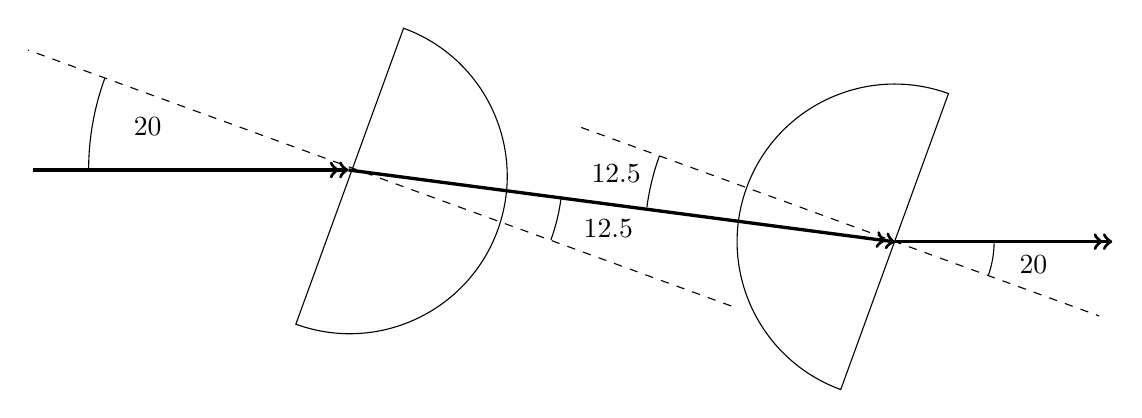
\begin{tikzpicture}
      
      % first incident ray
      \draw[->>,very thick] (0.3,0.2) -- (4.3,0.2);
      
      % first semi circle
      \draw[] (5,2) arc(70:-110:2) -- cycle;

      % normal of first semi circle
      \draw[dashed, rotate around={-20:(5,0.2)}] (9.5,0) -- (0,0);

      % origin line
      % \draw[dashed] (0,0.2) -- (20,0.2);

      % first angle of incidence
      \draw[] (1,0.2) arc(180:160:3.4);
      \path (1.75,0.75) node {\(\SI{20}{\degree}\)};
      
      % first refraction ray / second incidence ray
      \draw[->>, very thick, rotate around={-7.5:(4.3,0.2)}] (4.3,0.2) -- (11.3,0.2);
      
      % first angle of refraction
      \draw[] (7,-0.16) arc(-7.5:-20:2.5);
      \path (7.6,-0.55) node {\(\SI{12.5}{\degree}\)};

      % second angle of incidence
      \draw[] (8.25,0.38) arc(160:172.5:3.1);
      \path (7.7,0.16) node {\(\SI{12.5}{\degree}\)};

      % second semi circle
      \draw[] (11.92,1.17) arc(70:250:2) -- cycle;

      % normal of second semi circle
      \draw[dashed, rotate around={-20:(11.24,-0.71)}] (7,-0.71) -- (14,-0.71);
      
      % second refraction ray
      \draw[->>, very thick] (11.24,-0.71) -- (14,-0.71);

      % second angle of refraction
      \draw[] (12.5,-0.71) arc(0:-20:1.28);
      \path (13,-1) node {\(\SI{20}{\degree}\)};

    \end{tikzpicture}
  \end{center}
  \caption{A diagram showing the path of the ray through the flat end of the lens,
    followed by the curved end of the lens. The principle of optical reversibility
    is shown because the initial refraction of the light ray is undone be
    reversing the orientation of the lens.}
\end{figure}

\subsubsubsection{}

The principle of optical reversibility also holds for reflection. If the path of
a reflected ray is followed in reverse, the same path will be taken.

%-----------END EXPERIMENT 5-----------

%----------BEGIN EXPERIMENT 6----------

\subsection{Experiment 6: Dispersion and Total Internal Reflection}

\subsubsection{Dispersion}

\subsubsubsection{}

Color separation began to appear at around 20 degrees.

\subsubsubsection{}

The maximum amount of color separation appeared at around 40 degrees.

\subsubsubsection{}

In the refracted ray, red has the smallest angle of refraction, followed, in
ascending order, by yellow, green, blue, and purple.

\subsubsubsection{}

At an angle of incidence of 40 degrees, the angles of refraction for red light
and blue light are, respectively, \(\theta_{i,red} = \SI{76.5}{\degree}\) and
\(\theta_{i,blue} = \SI{85}{\degree}\). The index of refraction of the acrylic,
\(n_i\), can be found be rearranging Snell's Law,
\(n_r \sin{(\theta_r)} = n_i \sin{(\theta_i)}\), as
\(n_i = \frac{n_r \sin{(\theta_r)}}{\sin{(\theta_i)}}\), where
\(n_r = n_{air} = 1\) and \(\theta_i = \SI{40}{\degree}\).

The index of refraction of the acrylic for red light may be found with:

\begin{align*}
  n_{i,red} &= \frac{n_r \sin{(\theta_r)}}{\sin{(\theta_{i,red})}} \\
  n_{i,red} &= \frac{(1) \sin{(76.5)}}{\sin{(40)}} \\
  n_{i,red} &= 1.51 \\
\end{align*}

The index of refraction of the acrylic for blue light may be found with:


\begin{align*}
  n_{i,blue} &= \frac{n_r \sin{(\theta_r)}}{\sin{(\theta_{i,blue})}} \\
  n_{i,blue} &= \frac{(1) \sin{(85)}}{\sin{(40)}} \\
  n_{i,blue} &= 1.55 \\
\end{align*}

\subsubsection{Total Internal Reflection}

\subsubsubsection{}

While reflection off the flat edge is dim, the reflection from the curved edge
is much more prominent and complete at an incident angle of 80 degrees.

\subsubsubsection{}

Yes, there is always a reflected ray for all angles of incidence.

\subsubsubsection{}

Yes, the angles for the reflected rays are consistent with the Law of Reflection
because the incidence angles match the angles of the rays' reflection.

\subsubsubsection{}

There is not a refracted ray for all angles of incidence; there is no refracted
ray for angles of incidence above 45 degrees on the curved edge.

\subsubsubsection{}

As angle of incidence increases, the intensity of the refracted rays decreases,
while the intensity of the reflected rays increases.

\subsubsubsection{}

All the light is reflected at an angle of refraction of 83 degrees.

%-----------END EXPERIMENT 6-----------

%----------BEGIN EXPERIMENT 7----------

\subsection{Experiment 7: Converging Lens - Image and Object Relationships}

\subsubsection{Data}

\begin{figure}[H]
  \label{tab:7.1}
  \caption{\textbf{Table 7.1:} The data calculated from the experiment and the
    calculated values determined from the data. Calculations were performed by
    reading the data into a Julia DataFrame, then performing the requested
    operations on that data. The following formulas
    \(\frac{1}{f} = \frac{1}{d_o} + \frac{1}{d_i}\) and
    \(M = - \frac{d_i}{d_o} = \frac{h_i}{h_o}\) were used.}
  \begin{center}
    \begin{tabular}{|ccc|cccc|}
      \hline
      \multicolumn{3}{|c|}{Data (\si{\milli\meter})} &
      \multicolumn{4}{|c|}{Calculations} \\
      \hline
      \(d_o\) & \(d_i\) & \(h_i\) & 
      \(\frac{1}{d_i} + \frac{1}{d_o}\) (\si{\per\milli\meter}) &
      \(\frac{1}{f}\) (\si{\per\milli\meter}) &
      \(\frac{h_i}{h_o}\) &
      \(\frac{-d_i}{d_o}\) \\
      \hline
      50 & n/a & n/a & n/a    & n/a    & n/a    & n/a    \\
      75 & inf & n/a & n/a    & n/a    & n/a    & n/a    \\
      100 & 295 & 59 & 0.0140 & 0.0140 & -0.166 & -0.166 \\
      150 & 114 & 19 & 0.0137 & 0.0137 & -0.193 & -0.193 \\
      200 & 115 & 11 & 0.0137 & 0.0137 & -0.222 & -0.222 \\
      250 & 105 & 9  & 0.0136 & 0.0136 & -0.265 & -0.265 \\
      300 & 96 & 6.5 & 0.0137 & 0.0137 & -0.320 & -0.320 \\
      350 & 93 & 5.5 & 0.0135 & 0.0135 & -0.420 & -0.420 \\
      400 & 89 & 4.5 & 0.0136 & 0.0136 & -0.575 & -0.575 \\
      450 & 87 & 4   & 0.0154 & 0.0154 & -0.760 & -0.760 \\
      500 & 83 & 3.5 & 0.0133 & 0.0133 & -2.950 & -2.950 \\
      \hline
    \end{tabular}
  \end{center}
\end{figure}

\subsubsection{Questions}

\subsubsubsection{}

The image is magnified.

\subsubsubsection{}

The image is inverted.

\subsubsubsection{}

As \(d_o\) increases, \(d_i\) decreases.

\subsubsubsection{}

If \(d_o\) were very, very large, \(d_i\) would tend toward \(f\). Since \(d_o\)
is very large, \(\frac{1}{d_o} \rightarrow \frac{1}{\infty} \approx 0\), therefore,

\begin{align*}
  \frac{1}{f} &= \frac{1}{d_o} + \frac{1}{d_i} \\
  \frac{1}{f} &= (0) + \frac{1}{d_i} \\
  \frac{1}{f} &= \frac{1}{d_i} \\
  f &= d_i \\
\end{align*} 

\subsubsubsection{}

The focal length was determined by measuring the distance between the lens and
the view screen when a crisp image was shown on the view screen. The focal
length was measured to be \(\SI{8}{\centi\meter}\).

\subsubsubsection{}

The measurements appear to be in agreement with the Fundamental Lens Equation.

\subsubsubsection{}

We were unable to focus an image on the screen for \(d_o <
\SI{75}{\milli\meter}\). The focal point of the lens is
\(\SI{75}{\milli\meter}\), so, according to the Fundamental Lens Equation, when
\(d_o = f\), \(d_i = \infty\). We could not get a focused image at \(d_o =
\SI{50}{\milli\meter}\) because \(d_o < f\). 

%-----------END EXPERIMENT 7-----------

%----------BEGIN EXPERIMENT 8----------

\subsection{Experiment 8: Light and Color}

\subsubsection{The Colors of Light}

\subsubsubsection{}

Our observations support Newton's theory, because colors appeared from the white
light.

\subsubsubsection{}

When red, green, and blue light are mixed together, they produce white
light. This supports Newton's theory because it shows that white light must be
comprised of several colors, since the combination of those colors produces
white light.

\subsubsection{The Colors of Objects}

\subsubsubsection{}

The transmitted rays were green, and the reflected rays were white.

\subsubsubsection{}

The reflected rays are white. The green filter ought to reflect all rays except
green, which it transmits, and the red filter ought to reflect all rays except
red, which it transmits. All the reflected rays appeared to be white.

\subsubsubsection{}

Since we did not have a blue filter, we used the blue/green filter instead. The
reflected rays were blue.

\subsubsubsection{}

The green filter appears green because it absorbs and transmits only green light
while reflecting all other colors.

%-----------END EXPERIMENT 8-----------

%----------BEGIN EXPERIMENT 9----------

\subsection{Experiment 9: Two-Slit Interference}

\subsubsection{Data}

\begin{figure}[H]
  \label{tab:9.1}
  \caption{\textbf{Table 9.1:} The different parts of the slit geometry.}
  \begin{center}
    \begin{tabular}{|ccccc|c|}
      \hline
      \multicolumn{5}{|c|}{Data} & Calculations \\
      \hline
      Color & n & AB (\si{\centi\meter}) & X (\si{\centi\meter}) & L
                                                                   (\si{\centi\meter})
                                                                 & 
\(\frac{(AB)}{n} \sin{(\tan{}^{-1}(\frac{X}{L}))} = \lambda\) \\
      \hline
      red        & 5 & & 1   & 35 &   \\
      green      & 4 & & 0.5 & 35 &   \\
      blue/green & 7 & & 1   & 35 &   \\
      \hline
    \end{tabular}
  \end{center}
\end{figure}

%-----------END EXPERIMENT 9-----------

%----------BEGIN EXPERIMENT 10----------

\subsection{Experiment 10: Polarization}

\subsubsection{Polarization}

\subsubsubsection{}

The target does not appear bright because a significant portion of the light is
not making it through the polarizers.

\subsubsubsection{}

The light from the light source plane is not polarized because the light is
visible no matter the orientation of a single polarizer.

\subsubsubsection{}

A maximum amount of light is allowed through the polarizers when polarizer B is
at \(\SI{0}{\degree}\) and \(\SI{180}{\degree}\) because those angles align with
polarizer A. A minimum amount of light is allowed through when polarizer B is
perpendicular to polarizer A at angles \(\SI{90}{\degree}\) and
\(\SI{270}{\degree}\).

\subsubsection{Polarization by Reflection: Brewster's Angle}

\subsubsubsection{}

The reflected light is polarized. The light is bright at angles
\(\SI{0}{\degree}\) and \(\SI{180}{\degree}\), while it is dim at
\(\SI{90}{\degree}\) and \(\SI{270}{\degree}\).

\subsubsubsection{}

The light plane is not polarized when the reflected ray is not at an angle of
\(\SI{90}{\degree}\) with respect to the refracted ray, because the light is
visible for all angles of the polarizer. 

%-----------END EXPERIMENT 10-----------

%----------BEGIN EXPERIMENT 11----------

\subsection{Experiment 11: Image Formation from Cylindrical Mirrors}

\subsubsection{Procedure}

\subsubsubsection{}

The focal length of the concave cylindrical mirror was measured to be
\(\SI{61.5}{\milli\meter}\).

\subsubsubsection{}

The focal length of the convex cylindrical mirror was measured to be
\(\SI{6}{\centi\meter}\). 

\begin{figure}[H]
  \label{pic:exp11}
  \begin{center}
    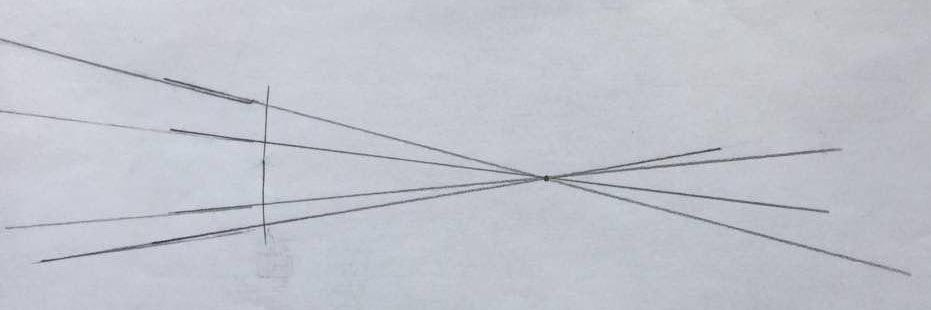
\includegraphics[scale=0.4]{exp11.jpg}
  \end{center}
  \caption{The ray trace of the light rays traveling through the convex mirror.}
\end{figure}

\subsubsection{Image Location}

\subsubsubsection{}

The image of the light bulb filament is formed where the reflected rays cross.

\subsubsubsection{}

The image is not noticeably affected by moving the mirror closer to the filament
until it gets very close, because the light rays then begin to diverge.

\subsubsubsection{}

An image is not formed when the distance between the filament and the mirror is
less than the focal length because the rays become divergent at lengths below
the focal length.

\subsubsubsection{}

A real image cannot be obtained from the convex side of the mirror because the
rays diverge from a convex mirror.

\subsubsection{Magnification and Inversion}

\subsubsubsection{}

The degree of magnification increases as the object distance, \(d_o\), decreases
because \(M = - \frac{d_i}{d_o}\).

\subsubsubsection{}

The image is inverted. The image inversion does depend on image location,
because if the image is viewed from beyond the focal point, the rays have
converged and crossed over each other, thus flipping the image.

\subsubsection{Cylindrical Aberration}

\subsubsubsection{}

The rays are all focused at the same point, but the rays closer to the edges are
less distinct.

\subsubsubsection{}

To reduce the amount of cylindrical aberration, the lens ought to be made into a
parabolic shape.

%-----------END EXPERIMENT 11-----------

%----------BEGIN EXPERIMENT 13----------

\subsection{Experiment 13: Image Formation with Cylindrical Lenses}

\subsubsection{Focal Point}

\subsubsubsection{}

\(f_1 = \SI{7}{\centi\meter}\) and \(f_2 = \SI{5.1}{\centi\meter}\)

\subsubsubsection{}

The refracted rays converge at the same focal length.

\subsubsubsection{}

The refracted rays now converge further than before. On the flat edge of the
lens, the rays are parallel until they exit, and on the curved edge of the lens,
the incident rays are never parallel. Since the rays are never parallel once
they contact the lens on the curved side, their focal length is shorter.

\subsubsection{Image Location}

\subsubsubsection{}

The image is formed at \(\SI{7}{\centi\meter}\).

\subsubsubsection{}

The image moves further away as the light source nears.

\subsubsubsection{}

No image is formed when the light source is closer than the lens' focal length.

\subsubsection{Magnification and Inversion}

\subsubsubsection{}

Magnification increases as the lens nears the light source.

\subsubsubsection{}

The image is inverted for all object locations.

\subsubsection{Cylindrical Aberration}

\subsubsubsection{}

All of the rays, except those at the edges, are focused at precisely the same
point.

%-----------END EXPERIMENT 13-----------

%----------BEGIN EXPERIMENT 14----------

\subsection{Experiment 14: Spherical Lenses - Spherical and Chromatic
  Aberration, Aperture Size, and Depth of Field}

\subsubsection{Spherical Aberration}

\subsubsubsection{}

The smaller the aperture, the greater the focus of the image.

\subsubsubsection{}

An infinitely small aperture would, theoretically, provide the best focus, but
it is impractical because not enough light would get through to sufficiently
illuminate the image.

\subsubsection{Depth of Field}

\subsubsubsection{}

The depth of field is reduced as the aperture size decreases.

\subsubsubsection{}

An infinitely long depth of field would produce a very blurry image.

\subsubsubsection{}

An image of the target is still visible on the screen after the lens is removed.

\subsubsubsection{}

As the size of the aperture increases, the distinctness of the image decreases.

\subsubsubsection{}

As the distance between the aperture and viewing screen increases, the
magnification of the image also increases.

\subsubsubsection{}

The very small aperture serves the role of focusing the light that passes
through it. This principle is exploited by pinhole cameras.

\subsubsection{Chromatic Aberration}

\subsubsubsection{}

Chromatic aberration is more apparent when the aperture is far from the optical
axis of the lens because there is more space for the rays to separate.

%-----------END EXPERIMENT 14-----------

%----------BEGIN EXPERIMENT 15----------

\subsection{Experiment 15: The Diffraction Grating}

\subsubsection{Data}

\begin{figure}[H]
  \label{tab:15.1}
  \caption{\textbf{Table 15.1:} The data needed to calculate the minimum and
    maximum wavelengths. \(A \sin{(\tan{}^{-1}(\frac{X}{L} = \lambda))}\)}
  \begin{center}
    \begin{tabular}{|ccccc|cc|}
      \hline
      \multicolumn{5}{|c|}{Data (\si{\centi\meter})} & 
      \multicolumn{2}{|c|}{Calculations (\si{\nano\meter})} \\
      \hline
      Color & A & L & \(X_1\) & \(X_2\) & \(\lambda_1\) & \(\lambda_2\) \\
      \hline
      violet & \num{0.00016} & 35 & 7.5  & 8.5  & 335 & 377 \\
      blue   & \num{0.00016} & 35 & 8.5  & 10.5 & 377 & 459 \\
      green  & \num{0.00016} & 35 & 10.5 & 11.7 & 459 & 507 \\
      yellow & \num{0.00016} & 35 & 11.7 & 12.3 & 507 & 530 \\
      orange & \num{0.00016} & 35 & 12.3 & 13   & 530 & 557 \\
      red    & \num{0.00016} & 35 & 13   & 15   & 557 & 630 \\
      \hline
    \end{tabular}
  \end{center}
\end{figure}

\subsubsection{Questions}

\subsubsubsection{}

As slit width increases, the width of the maxima also increases.

\subsubsubsection{}

The high number of slits creates a thin pattern with many lines close together.

%-----------END EXPERIMENT 15-----------

%----------BEGIN EXPERIMENT 16----------

\subsection{Experiment 16: Single Slit Diffraction}

\subsubsection{Questions}

\subsubsubsection{}

The narrower the slits, the narrower the fringes.

\subsubsubsection{}

The single slit, pattern A, produces a narrow, blurry patter, while the
double slit, pattern D, produces a spread out, distinct pattern.

%-----------END EXPERIMENT 16-----------

%----------BEGIN EXPERIMENT 19----------

\subsection{Experiment 19: The Projector}

\subsubsection{Questions}

\subsubsubsection{}

The image cannot be focused onto the viewing screen when \(d_o < f\) because the
rays diverge.

\subsubsubsection{}

The image can be focused when \(d_o > 2f\) because the rays are able to
converge.

\subsubsubsection{}

In order for substantially large magnification, \(d_o < f\), which is not
practical because an image is not produced. It is impossible to project an
uninverted image with only a single lens.

\subsubsubsection{}

The image formed by a projector cannot be viewed without a viewing screen.

%-----------END EXPERIMENT 19-----------

%----------BEGIN EXPERIMENT 20----------



%-----------END EXPERIMENT 20-----------

%----------BEGIN EXPERIMENT 21----------



%-----------END EXPERIMENT 21-----------

%----------BEGIN EXPERIMENT 22----------



%-----------END EXPERIMENT 22-----------

%----------BEGIN CONCLUSION----------

\section{Conclusion}

\qq Almost all of our data matches with theory. The data collected for
Experiment 2 is entirely correct. Experiment 4's data is a bit less precise, but
it is very close to its theoretical value, because the points very nearly match
the lines of best fit. The data for Experiment 5 is very near what it is
supposed to be; the data has no discrepancy higher than 6\%. Error throughout
the experiments may be contributed to our inability to perfectly align the lab
equipment and limitations encountered during measurement.

%-----------END CONCLUSION-----------

\end{document}
